\documentclass[a4paper,12pt,oneside,onecolumn]{article}
\usepackage[utf8]{inputenc}
\usepackage{graphicx}
\usepackage[round,numbers]{natbib}
\usepackage{hyperref}
\usepackage{amsmath}
\usepackage{listings}
\usepackage[T1]{fontenc}
\usepackage[scaled=0.9]{beramono}
\usepackage{microtype}
\usepackage{color}
\usepackage{xcolor}
\usepackage{lipsum}
\usepackage{float}
\usepackage[italian]{babel}

\usepackage[noadvisor,swapnames]{frontespizio}

\begin{document}


\begin{frontespizio}
\Universita {Bari "Aldo Moro"}
\Logo [2cm]{./images/logo}
\Dipartimento{Informatica}
\Corso [Laurea]{Informatica Magistrale}
\Titoletto {Documentazione di progetto di Intelligenza Artificiale}
\Titolo{Text Extraction in ambito giuridico}
\NCandidato{Studenti}
\Candidato{Luciano Quercia}
\Candidato{Simone Rutigliano}
\Annoaccademico {2013-2014}
\Margini{4cm}{4.5cm}{4cm}{4cm}
\end{frontespizio}


\nocite{mirizzilinked}


%\section{Introduzione}

Il nostro progetto consiste nella realizzazione di un content-based recommender system che raccomandi film utilizzando dati provenienti dalla Linked Open Data Cloud al fine di poter aumentare l'efficienza del recommender system utilizzando informazioni aggiuntive inerenti un particolare film utilizzando differenti fonti.

\subsection{Linked Data}
L’interoperabilità è uno dei vantaggi più importanti del modello Open Data. I dati, se isolati, hanno poco valore; viceversa, il loro valore aumenta sensibilmente quando data set differenti, prodotti e pubblicati in modo indipendente da diversi soggetti, possono essere incrociati liberamente da terze parti. Questo è alla base del processo di creazione di valore aggiunto sui dati: le applicazioni. Le applicazioni, di valore sociale e/o economico, sfruttano quello che può essere visto come un grande database aperto e distribuito per offrire viste e servizi. L’interoperabilità è dunque un elemento chiave di uno degli aspetti più innovativi offerti dagli open data: l’uso dei dati in modi e per scopi “inattesi”, nuovi in quanto non previsti dai singoli enti e soggetti che pubblicano i “dati grezzi”.

Occorre cioè collegare i dati tra loro, stabilendo un link diretto quando i dati (possibilmente provenienti da diverse sorgenti) si riferiscono a oggetti identici o comunque relazionati tra loro. Tale collegamento diretto si manifesta come la possibilità di “saltare” da un dataset all’altro, ad esempio quando si vuole accedere a dati (come i dettagli su una particolare entità) che non si posseggono al’interno.
Supponiamo per esempio di avere, da una parte, amministrazioni locali che pubblicano dati aperti relativi ai monumenti storici e agli hotel che si trovano nelle vicinanze di quei monumenti; dall’altra, Sovrintendenze ai Beni Culturali che pubblicano dati dettagliati sui monumenti, gli artisti e i periodi storici, e sui quadri esposti nei musei o nei palazzi.
Combinare i due dataset potrebbe essere di grande utilità, ad esempio per offrire un servizio personalizzato sugli itinerari in base agli interessi culturali specifici di un turista.

Nei cosiddetti Linked Data, questi collegamenti e relazioni tra le entità descritte nei dataset sono espliciti.
\subsection{Machine readable vs. machine linkable}
I linked data, per definizione, vengono espressi tramite Resource Description Framework (RDF). RDF non è propriamente un formato di dati, ma un “data model”, cioè un formalismo per rappresentare dati. Un dataset RDF può essere infatti serializzato in diversi formati (RDF/XML, N3, NTriple, etc.), ma il data model RDF possiede alcune caratteristiche che restano immutate, a prescindere dal formato che viene utilizzato.

In poche parole il modello RDF è costituito da triple, della forma soggetto-predicato-oggetto. Le triple possono condividere oggetto o soggetto così da formare un grafo.

\begin{figure}[htbp]
  \centering
  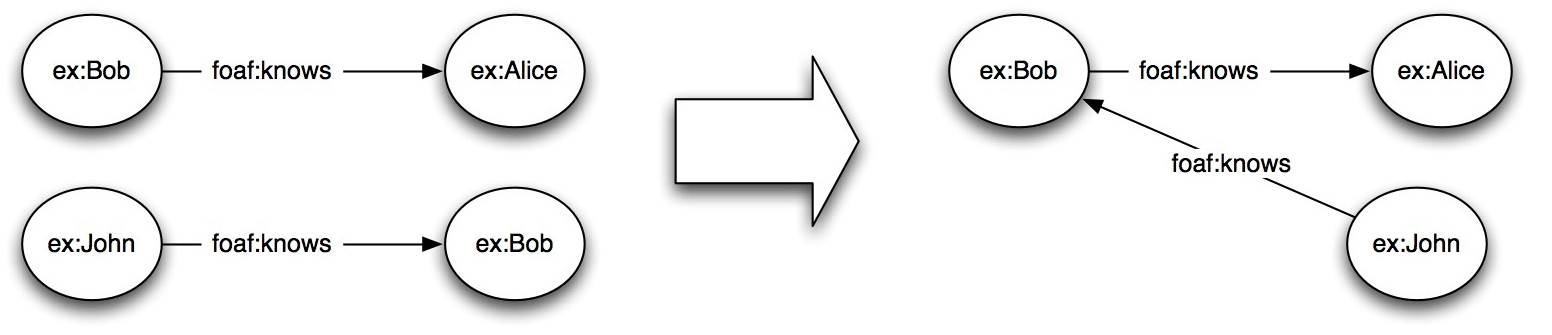
\includegraphics[width=.9\textwidth]{./images/triples1-crop}
\end{figure}

Questo insieme di triple RDF (o grafo) può essere espresso, allo scopo di essere scambiato tra applicazioni e pubblicato sul web, in vari formati di serializzazione.

\clearpage

Ad esempio in RDF/XML:

\begin{lstlisting}
<?xml version="1.0"?>
<rdf:RDF
    xmlns:ex="http://example.org/"
    xmlns:foaf="http://xmlns.com/foaf/0.1//"
    xmlns:rdf="http://www.w3.org/1999/02/22-rdf-syntax-ns#">
    <rdf:Description rdf:about="http://example.org/John">
        <foaf:knows>
            <rdf:Description rdf:about="http://example.org/Bob">
                <foaf:knows rdf:resource="http://example.org/Alice" />
            </rdf:Description>
        </foaf:knows>
    </rdf:Description>
</rdf:RDF>
\end{lstlisting}


La caratteristica più importante di tale modello, che si sposa con la visione Linked Data, è usare Uniform Resource Identifier (URI).

Tornando all’esempio del monumento, supponiamo che i due dataset (amministrazione locale e sovrintendenza) siano stati pubblicati come Linked Data. Per identificare i monumenti, il dataset delle sovrintendenza usa URL (del tipo \emph{http://cultural-heritage-example.org/monument/XYZ}). Il contenuto digitale di tali URL corrisponde alla descrizione dettagliata dei monumenti.
Il data set dell’amministrazione locale, inserendo dei link a tali URL, come avviene in figura 1, permetterebbe a un software di risolvere l’URL e ottenere la descrizione del monumento (sempre aggiornata).

Ancora, dal momento che RDF consente di specificare precisi tipi di risorse, potremmo pensare a un semplice script che trovi tutte le risorse di tipo “monumento” nel dataset dell’amministrazione locale, e che importi, per ciascuna, informazioni aggiuntive, creando così un dataset misto. Su quest’ultimo nuovodata set arricchito, si potrebbero poi fare query del tipo “trova tutti gli alberghi vicini a un monumento successivo al XIII secolo, in cui siano esposte sculture del Canova”.

\floatplacement{figure}{H}
\begin{figure}
\centering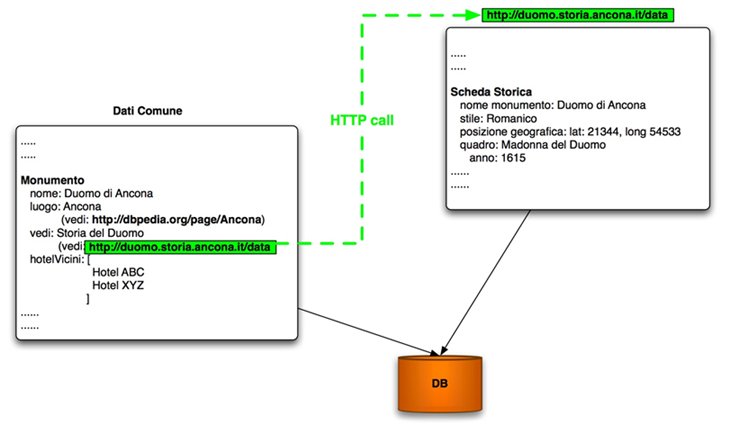
\includegraphics[width=.8\textwidth]{./images/img2}
\end{figure}
Questo esempio è solo uno degli scenari possibili in cui i linked data possono favorire l’interoperabilità tra dataset. Le possibilità sono infinite se pensiamo alla vasta quantità di Linked Open Data già presenti sul Web. \textbf{DBPedia.org}, per esempio, espone una grande porzione di dati di Wikipedia come linked data, mentre \textbf{Geonames} offre descrizioni RDF di entità geografiche. \emph{http://linkeddata.org/} fornisce un quadro dello stato corrente della “Linked data cloud”, e mostra un ecosistema di database interconnessi in rapida crescita.

%\section{Lavori correlati}
\label{relatedworks}

In \citet{mirizzilinked}, affrontando lo stesso problema, è stato utilizzato un VSM puro, trasformando il grafo RDF di partenza in un tensore 3-dimensionale di adiacenza.

Nel 2008, in \citet{passant2008combining}, gli autori introducevano la possibilità di utilizzare i Linked Open Data sia in un contesto di collaborative filtering (utilizzando il vocabolario \verb+foaf+) sia in recommender content-based (con le informazioni provenienti da \emph{dbpedia} e \emph{dbtune}).

In \citet{passant2009using}, gli autori effettuano un confronto tra un sistema di raccomandazione di tipo content-based attraverso l'utilizzo dei lod e un sistema di collaborative filtering.

In \citet{passant2010measuring}, invece, in un contesto differente dal nostro (artisti musicali), sono state introdotte le misure che verranno spiegate in seguito (\ref{measures}) e che verranno utilizzate come baseline per le nostre sperimentazioni. 

\nocite{freitas2012distributional}




\nocite{thalhammer2012leveraging}

%\section{Progetto}
\label{project}

Il progetto è composto da 5 sezioni:
\begin{itemize}
\item\emph{graph}
\item\emph{distance}
%\item\emph{movielens\_exp}
\item\emph{profile}
\item\emph{recommendation}
\end{itemize}

\subsection{graph}
Nella parte iniziale del progetto verranno eseguiti dei metodi presenti nella classi situate all'interno del package \emph{graph}, i cui scopi saranno quelli di:
\begin{itemize}
\item Salvare all'interno di un grafo i film presenti nel db di movielens;
\item A partire dal grafo creato in precedenza, si va a creare un nuovo grafo in cui ogni vertice rappresenta un film, mentre ogni arco rappresenta un possibile collegamento che intercorre tra due film attraverso un qualunque tipo di risorsa quale ad esempio un particolare attore facente parte del casting di entrambi i film presi in considerazione.
\end{itemize}

Al fine di soddisfare il primo obiettivo, all'interno della classe \textsc{Graph} sarà presente un metodo atto alla creazione del multigrafo sparso non direzionato attraverso l'esecuzione di query SPARQL utilizzando come endpoint il link di Dbpedia (\textit{http://dbpedia.org/sparql}).

Il risultato di questa computazione sarà un multigrafo avente come vertice risorse quali film,attori,case produttrici,registi,ecc; mentre come arco un predicato che mette in relazione le due risorse quale ad esempio director,writer,music composer e cosi via.

Per quanto riguarda il secondo obiettivo,all'interno della classe \textsc{FilmGraph} sarà presente un metodo il cui scopo sarà quello di convertire il multigrafo sparso non direzionato, in un nuovo multigrafo sparso direzionato i cui vertici saranno solo i film presenti nel db di movielens, mentre i cui archi saranno creati relazionando tra loro due archi definiti in precedenza aventi come soggetto della prima proprietà il film di partenza e come oggetto della seconda proprietà il film di destinazione.

\subsection{distance}
Il compito principale di questo package è quello di creare sia tutte le distanze di passant (verranno definite nel dettaglio nei paragrafi \ref{PassantD} e \ref{PassantC}), sia le distanze da noi implementate (\ref{PassantDW} e \ref{PassantCW}).

\subsection{profile}
Tramite le classi presenti all'interno di questo package, sarà possibile implementare le due tipologie di profilo (pesato e non pesato)(verranno descritte in dettaglio nel paragrafo \ref{profili}).

\subsection{recommendation}
Come dice il nome stesso, il compito di questo package consiste nella vera e propria fase di raccomandazione ad un utente partendo da una particolare configurazione. Per configurazione si intende definire innanzitutto ia tipologia di \emph{\textbf{distanza}} da utilizzare, poi si va definire quale tipo di profilo utente utilizzare (\emph{\textbf{pesato}} o \emph{\textbf{non pesato}}) e infine il numero \emph{\textbf{k}} di raccomandazioni da fare.

%\subsection{movielens\_exp}
%Il package \emph{movielens\_exp} ha il compito di eseguire la fase sperimentale del progetto; innanzitutto viene eseguita la fase di splitting delle votazioni date da ogni utente ai vari film visionati allo scopo di creare i set di training e di test. Successivamente si passa alla creazione dei profili(\emph{pesato} e \emph{non pesato}) partendo dalle votazioni presenti all'interno del training set di ogni utente; infine nella parte finale della sperimentazione vengono calcolate le diverse tipologie di metriche descritte in \ref{metriche}.


%\section{Misure}
\label{measures}

\subsection{Distanze}

Il nostro recommender system è stato testato su quattro diverse misure di distanza.
Le prime due sono descritte in \citet{passant2010measuring}, le altre due sono state realizzate \emph{ex novo} e rappresentano una nuova visione pesata delle precedenti.


\subsubsection{Passant Direct}
\label{PassantD}
La distanza diretta. Indica il numero di archi diretti che collegano i film $a$ e $b$. Tenendo conto che il grafo preso in considerazione è orientato, vanno presi gli archi in entrambe le direzioni.

In maniera formale, definita $$C_{d}(f_a,f_b) = \left\vert \left\{ e \in Edges \  | \  (f_a \xrightarrow{~e~} f_b ) \right\} \right\vert$$ la formula della distanza completa sarà quindi:

%\begin{figure}[htbp]
%  \centering
%    \label{LDSD}
%    \begin{equation}
%        P_{d}(r_{a},r_{b}) = \frac{1} {1+C_{d}(n,r_{a},r_{b})+C_{d}(n,r_{b},r_{a})}
%    \end{equation}
%      \caption{LDSD Distance}
%      \label{LDSD1}
%\end{figure}

    \begin{equation}
        P_{d}(f_{a},f_{b}) = \frac{1} {1+C_{d}(f_{a},f_{b})+C_{d}(f_{b},f_{a})}
    \end{equation}

\subsubsection{Passant Combinated}
\label{PassantC}

La distanza combinata compone la precedente distanza diretta con una misura
(PassantI) che prende in considerazione i percorsi che uniscono due film
attraverso un film in comune.

PassantI restituisce un valore che indica il numero di archi che
mettono in relazione i due film attraverso dei film in comune.

Formalmente, definiti:
$$C_{io}(f_a,f_b) = \left\vert \left\{ f \  | \  (f_a \xrightarrow{~e~} f ) \wedge (f_b \xrightarrow{~e~} f) \right\} \right\vert$$
$$C_{ii}(f_a,f_b) = \left\vert \left\{ f \  | \  ( f \xrightarrow{~e~} f_a ) \wedge ( f \xrightarrow{~e~} f_b) \right\} \right\vert$$
$$\text{con} \ e \in Edges  , \qquad f_a,f_b,f \in Films $$

la formula indiretta di Passant è:
    \begin{equation*}
        P_i(f_{a},f_{b}) = \frac{1} {1+C_{io}(f_{a},f_{b})+C_{ii}(f_{a},f_{b})}
    \end{equation*}

La formula combinata sarà:

    \begin{equation}
P_{c}(f_{a},f_{b}) = \frac{1} {1+C_{d}(f_{a},f_{b})+C_{d}(f_{b},f_{a})+C_{io}(f_{a},f_{b})+C_{ii}(f_{a},f_{b})}
    \end{equation}


\subsubsection{Passant Direct Weighted}
\label{PassantDW}
La distanza diretta pesata, realizzata da noi, è una variazione della distanza diretta descritta in \ref{PassantD} che, invece che contare il numero di archi, somma i pesi di ciascun arco.

In maniera formale, dati:

\begin{equation*}
ED_{f_a,f_b} = \left\{ e \in Edges \quad\big\vert\quad f_a \xrightarrow{~e~} f_b \right\}\qquad\footnote{Ricordando che, nel nostro caso, trattandosi di un multigrafo, possono esserci più archi a collegare $f_a$ e $f_b$}
\end{equation*}

\begin{equation*}
CW_{d}(f_a,f_b) = \sum_{e \in ED}^{}{weight(e)}
\end{equation*}

\begin{equation}
P_{dw}(f_a,f_b) = \frac{1}{1+CW_{d}(f_a,f_b)+CW_{d}(f_b,f_a)}
\end{equation}

\subsubsection{Passant Combinated Weighted}
\label{PassantCW}
La distanza combinata pesata utilizza la precedente diretta pesata
\ref{PassantDW} insieme con la distanza che prende in considerazione i percorsi che uniscono due film attraverso un film in comune.

La distanza combinata, quindi, prende in considerazione sia gli archi diretti che gli archi indiretti (quelli che uniscono i film $a$ e $b$ passando da un film $c$ comune, come descritto in \ref{PassantC}). In questo caso, tuttavia, tutti gli archi sono pesati e la distanza corrisponde ad una sommatoria di pesi.

In maniera formale, dati
\begin{eqnarray*}
E'_{f_a,f_b} = & \left\{ (e_1, e_2) \in Edges ~ \big\vert ~ (f_a \xrightarrow{e_1} f_c) \wedge (f_b \xrightarrow{e_2} f_c) \wedge label(e_1)=label(e_2) \right\} \\
E''_{f_a,f_b} = & \left\{ (e_1, e_2) \in Edges ~ \big\vert ~ (f_c \xrightarrow{e_1} f_a) \wedge (f_c \xrightarrow{e_2} f_b) \wedge label(e_1)=label(e_2) \right\}
\end{eqnarray*}

\begin{eqnarray*}
CW_{io}(f_a,f_b) = \sum_{(e_1,e_2) \in E'_{f_a,f_b}}{weight(e_1)*weight(e_2)}\\
CW_{ii}(f_a,f_b) = \sum_{(e_1,e_2) \in E''_{f_a,f_b}}{weight(e_1)*weight(e_2)}
\end{eqnarray*}

\begin{equation*}
P_{cw}(f_{a},f_{b}) = \frac{1} {1+CW_{d}(f_a,f_b)+CW_{d}(f_b,f_a)+CW_{io}(f_a,f_b)+CW_{ii}(f_a,f_b)}
\end{equation*}

\subsection{Rappresentazione dei profili utente}
\label{profili}

Ogni utente deve essere profilato per poter registrare i suoi interessi,
affinché gli si possano raccomandare nuovi film corretti.
Per fare questo abbiamo sviluppato due tipi di rappresentazione dell'utente.
Il primo, più semplice, è il \emph{profilo non pesato}. In esso rappresentiamo i film visti in due insiemi, positivi e negativi. Il primo insieme viene utilizzato per migliorare le raccomandazioni mentre il secondo solo per tenere traccia dei film già visti e non raccomandarli nuovamente.
Il secondo è il \emph{profilo pesato}. In esso si tiene traccia di tutti i film
visti e del loro voto, in modo da pesare la loro influenza sul calcolo della
distanza. I film valutati positivamente influiranno avvicinando le potenziali raccomandazioni al profilo, tanto più quanto maggiore sarà il voto ricevuto. I film valutati negativamente, invece, aumenteranno la distanza.
Il peso dato a ciascun film del profilo sarà quindi pesato in relazione al voto ricevuto secondo la formula:
$$
P_{NORM}(f_a) = Voto(f_a)- Voto_M
$$

In una scala di $n$ valori, essi verranno traslati nell'intervallo $\left[-\frac{n}{2};\frac{n}{2}\right]$

%\section{Sperimentazione}
\label{experiment}

La sperimentazione è stata condotta utilizzando il dataset MovieLens, già noto in letteratura.
Il dataset è composto da 518 film e 613 utenti. Ciascun utente ha votato più film, con una votazione che va da 1 a 5.

Il protocollo sperimentale utilizzato nel progetto, prevede i seguenti passi:
\begin{enumerate}
\item Split del set di ogni utente secondo la proporzione 70/30 (il 70\% del set verrà utilizzato come Training Set, il restante 30\% come Test Set);
\item Per ogni utente:
    \begin{enumerate}
        \item Si creano i due profili utente (pesato e non pesato) utilizzando solo i dati presenti nel suo Training set;
        \item Si creano le liste di raccomandazioni, contenente la totalità dei film, ordinate per importanza, secondo le diverse tipologie di distanza definite nel capitolo \ref{measures};
    \end{enumerate}
\item $\forall k \in (5,10,20,50,100)$ , calcolo della Precisione $P_k$ (\ref{precision}), e del valore MRR (\ref{MRR}) tenendo conto anche delle diverse distanze calcolate e dei diversi profili costruiti in precedenza;
\end{enumerate}
Formalmente, possiamo dire che, l'esperimento controllato che verrà eseguito sarà un esperimento avente $n$ fattori con $m$ livelli, in particolare avremo 3 fattori:
\begin{itemize}
\item \textbf{Distanza} con 4 livelli: 
    \begin{itemize}
        \item \emph{Passant D} (\ref{PassantD}),
        \item \emph{Passant C} (\ref{PassantC}),
        \item \emph{Passant DW} (\ref{PassantDW}),
        \item \emph{Passant CW} (\ref{PassantCW});
    \end{itemize}
\item \textbf{Profilo} con 2 livelli (\ref{profili}) : 
    \begin{itemize}
        \item \emph{Pesato},
        \item \emph{Non Pesato};    
    \end{itemize}
\item \textbf{Numero di raccomandazioni $k$} con 5 livelli:
    \begin{itemize}
        \item \emph{5},
        \item \emph{10},
        \item \emph{20},
        \item \emph{50},
        \item \emph{100}.
    \end{itemize}
\end{itemize}
\subsection{Metriche}
\label{metriche}
Al fine di valutare la bontà del sistema creato abbiamo calcolato due tipologie di metriche:
\begin{itemize}
\item Precision
\item MRR
\end{itemize}
Per entrambe le tipologie sono stati presi in esame due punti di vista differenti (\emph{macroscopico} e \emph{microscopico}) ed inoltre, per ogni punto di vista, si è lavorato su due versioni differenti dello stesso dataset (\emph{epurato} e \emph{non epurato}). Questo è stato necessario al fine di migliorare le metriche relative alle raccomandazioni in quanto, nella valutazione, si vanno a considerare solo ed esclusivamente film presenti nel test set (\emph{epurato}) e non nell'intera totalità dei film presenti, di cui nella maggior parte dei casi (film non presenti nel test set) non conosciamo l'opinione dell'utente su quel particolare film (\emph{non epurato}).

\subsubsection{Precision}
\label{precision}
In un processo di classificazione statistica, la \emph{precisione} per una classe è il numero di \emph{true positive} (il numero di oggetti etichettati correttamente come appartenenti alla classe) diviso il numero totale di elementi etichettati come appartenenti alla classe (la somma di \emph{true positive} e \emph{false positive}, che sono oggetti etichettati erroneamente come appartenenti alla classe).
Inoltre i termini true positive, true negative, false positive e false negative sono usati per confrontare la classificazione di un oggetto (l’etichetta di classe assegnata all’oggetto da un classificatore) con la corretta classificazione desiderata (la classe a cui in realtà appartiene l’oggetto).
\begin{equation*}
Precision =\frac{TP}{TP+FP}
\end{equation*}

\paragraph{MicroPrecision}
Nel calcolo della microprecisione, è necessario prendere in considerazione i singoli valori di true positive e di false positive di ogni singolo utente come descritto nella formula:
\begin{equation*}
MicroPrecision =\frac{\sum\limits_{u\in U}^{}TP_u}{\sum\limits_{u\in U}^{}TP_u+\sum\limits_{u\in U}^{}FP_u}
\end{equation*}

\paragraph{MacroPrecision}
Per quanto riguarda invece il calcolo della macroprecisione, si va a prendere in considerazione il valor medio delle singole precisioni definite a livello di utente. Formalmente può essere descritto secondo la formula:
\begin{equation*}
MacroPrecision =\frac{1}{|U|}\sum\limits_{u\in U}{Precision_u}
\end{equation*}

\subsubsection{MRR}
\label{MRR}
Il Mean Reciprocal Rank (MRR) è un indice statistico per valutare un processo che produce una lista di possibili risposte ad una interrogazione (query), ordinate per probabilità di correttezza.
\begin{equation*}
MRR = \frac{1}{|Q|}\sum_{i=1}^{Q}{\frac{1}{Rank_i}}
\end{equation*}

\paragraph{MicroMRR}
Nel calcolo della microMRR, è necessario prendere in considerazione i singoli ranking delle raccomandazioni fatte ad ogni utente come descritto nella formula:
\begin{equation*}
MicroMRR =\frac{\sum\limits_{i=1}^{|R|}{\frac{relevant(r_i)}{i}}}{\sum\limits_{i=1}^{|R|}{\frac{1}{i}}} \qquad relevant(r_i)=\begin{cases} 1 & \mbox{se }r_i\mbox{ è rilevante} \\ 0 & \mbox{altrimenti}
\end{cases}
\end{equation*}
\paragraph{MacroMRR}
Per quanto riguarda invece il calcolo della macroMRR, si va a prendere in considerazione il valor medio dei singoli MRR definiti a livello di utente. Formalmente può essere descritto secondo la formula:
\begin{equation*}
MacroMRR =\frac{1}{|U|}\sum_{u\in U}{MRR_u}
\end{equation*}



\bibliographystyle{abbrvnat}
\bibliography{mybib}

\end{document}
